%Fiquemos com Deus e Nossa Senhora!
%Sao Jose de Cupertino rogai por nos!!
% ### Uses XeLaTeX ### %
% ### Needs beamer-master ### %
\documentclass[aspectratio=169]{beamer} %. Aspect Ratio 16:9

\usetheme{AI2} % beamerthemeSprace.sty
\usepackage[portuguese]{babel}
\usepackage[utf8]{inputenc}
\usepackage[T1]{fontenc}
\usepackage{ragged2e,gensymb}

\DeclareMathOperator*{\argmin}{arg\,min}
\DeclareMathOperator*{\argmax}{arg\,max}
\DeclareMathOperator{\sign}{sgn}

% DATA FOR FOOTER
\date{2021}
\title{- $k$-Médias}
\author{João Paulo Papa}
\institute{Advanced Institute for Artificial Intelligence (AI2)}

\begin{document}
% ####################################
% FIRST SLIDE 						:: \SliTit{This is the Title of the Talk}{A. B. Name}{Sprace}
% SUB-TITLE SLIDE 					:: \SliSubTit{<title>}{<explanation}
% SUB-SUB-TITLE SLIDE				:: \SliSubSubTit{<title>}{<explanation}
% SLIDE WITH TITLE 					:: \SliT{Title}{Content}
% SLIDE NO TITLE 						:: \Sli{Content} 
% SLIDE DOUBLE COLUMN WITH TITLE 	:: \SliDT{Title}{First Column}{Second Column}
% SLIDE DOUBLE COLUMN NO TITLE 		:: \SliD{First Column}{Second Column}
% SLIDE ADVANCED WITH TITLE 			:: \SliAdvT{Title}{Content}
% SLIDE ADVANCED NO TITLE 			:: \SliAdv{Content}
% SLIDE ADVANCED DOUBLE WITH TITLE 	:: \SliAdvDT{Title}{First Column}{Second Column}
% SLIDE ADVANCED DOUBLE NO TITLE 	:: \SliAdvD{First Column}{Second Column}
% SLIDE BLACK						:: \Black{ <Content> }
% SLIDE WHITE						:: \White{ <Content> }
% ITEMIZATION 						:: \begin{itemize}  \iOn{First} \iTw {Second} \iTh{Third} \end{itemize}
% COMMENT TEXT				 		:: \note{<comment>}
% SECTION 							:: \secx{Section} | \secxx{Sub-Section}
% BOLD SPRACE COLOR				:: \bfs{<text>}
% TABLE OF CONTENT					:: \tocitem{<title>}{<content>}
% LEFT ALIGN EQUATION				:: \begin{flalign*}  & <equation> &   \end{flalign*}
% CENTER ALIGN EQUATION	S			:: \begin{gather*} <equations>  \end{gather*}
% SLASH								:: \slashed{<>}
% BAR								:: \barr{<letter>} instead of \bar{<letter>}
% THEREFORE						:: use \portanto (larger and bold}
% 2 or 3 MATH SYMBOLS				:: \overset{<up>}{<down>} &  \underset{<below>}{\overset{<above>}{<middle>}}  
% INSERT TEXT IN FORMULA			:: \ins{<text>}
% EXERCISE							:: \exe{<exercise #>}{<exercise text>}
% SUGGESTED READING BOX			:: \sug{<references>}
% CITATION							:: \cittex{<citation>}
% CITATION DOUBLE COLUMN 			:: \cittexD{<citation>}
% TEXT POSITION						:: \texpos{<Xcm>}{<Ycm>}{<text>} origin = center of slide : x right | y down
% REFERENCE AT BOTTOM  S/D SLIDE		:: \refbotS{<reference>} \refbotD{<reference>}
% HIDDEN SLIDE						:: \hid
% COLOR BOX 						:: \blu{blue} + \red{rec} + \yel{yellow} + \gre{green} + \bege{beige}
% FRAME 							:: \fra{sprace} \frab{blue} \frar{red} + \fray{yellow} + \frag{green}		
% FIGURE 							:: \img{X}{Y}{<scale>}{Figure.png} 
% FIGURE							:: \includegraphics[scale=<scale>]{Figures/.png}
% FIGURE DOUBLE SLIDE NO TITLE		::  \img{-4}{0.5}{<scale>}{Figure.png} % Image 1st half
%									::  \img{4}{0.5}{<scale>}{Figure.png} % Image 2nd half
% FIGURE DOUBLE SLIDE WITH TITLE		::  \img{-4}{0}{<scale>}{Figure.png} % Image 1st half
%									::  \img{4}{0}{<scale>}{Figure.png} % Image 2nd half
% INCLUDING SWF (Flash)				:: \usepackage{media9} and \includemedia >> USE ACROBAT <<
%%%%%%%%%%%%%%%%%%%%%%%%%%%%%%%%%%%%%%%%%%%%%%%%%%
% ###############################################################################
% FIRST SLIDE
\SliTit{{\LARGE $k$-Médias}}{Advanced Institute for Artificial Intelligence -- AI2}{https://advancedinstitute.ai}
%%%%%%%%%%%%%%%%%%%%%%%%%%%%%%%%%%%%%%%%%%%%%%%%%%
% ###############################################################################
% SLIDE SUB-TITLE
%\SliSubTit{Sub-Title}{Description}{}
%%%%%%%%%%%%%%%%%%%%%%%%%%%%%%%%%%%%%%%%%%%%%%%%%%
% ###############################################################################
%\SliSubSubTit{Sub-Sub-Title}{Description}
 %%%%%%%%%%%%%%%%%%%%%%%%%%%%%%%%%%%%%%%%%%%%%%%%%%


\SliT{Introdução}{

\justifying Existem problemas para os quais não temos acesso aos rótulos da classes , ou seja, temos um problema de \textbf{aprendizado não supervisionada} (agrupamento). Nestas situações, não observamos os rótulos das amostras, tendo apenas um conjunto de dados definido da seguinte forma: ${\cal X} = \{\boldsymbol{x}_1,\boldsymbol{x}_2,\ldots,\boldsymbol{x}_m\}$, em que $\boldsymbol{x}_i\in\mathbb{R}^n$.

\begin{center}
	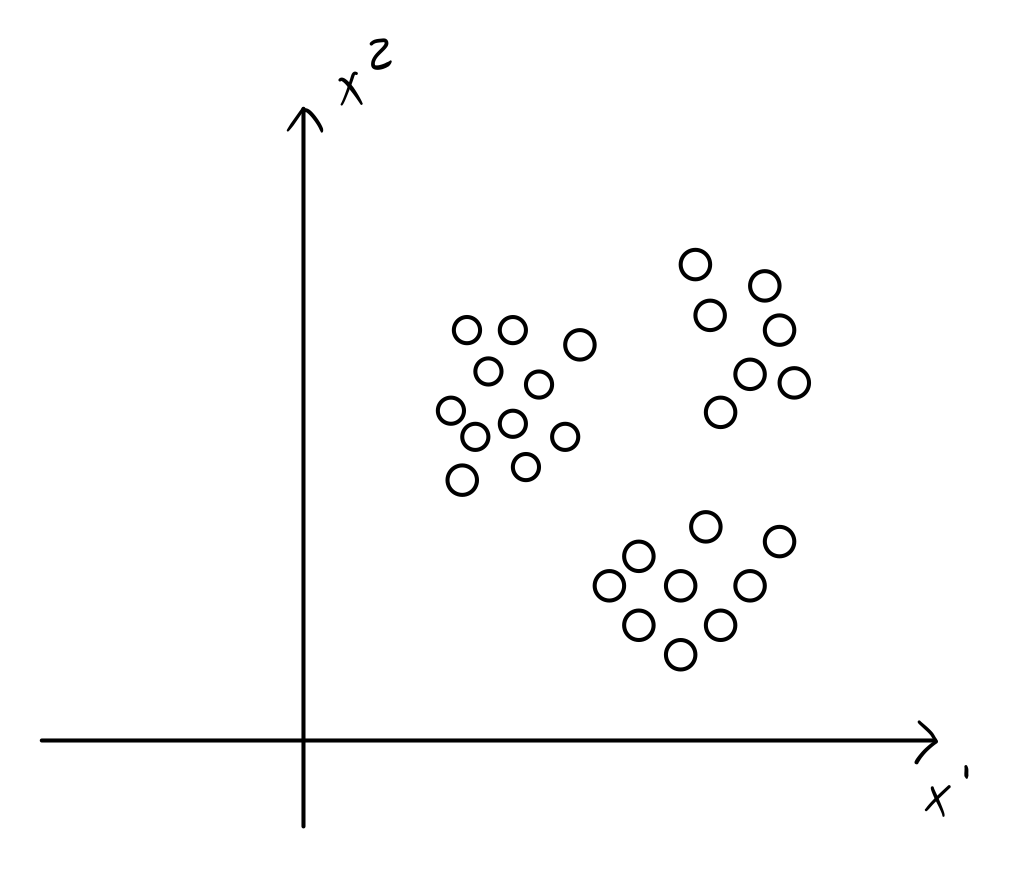
\includegraphics[scale=0.147]{./figs/KMeans_Fig1.png}
\end{center}

}

\Sli{
\justifying Uma das abordagens mais conhecidas é a chamada de $k$-Médias, do inglês \emph{$k$-Means}, a qual objetiva agrupar dados com base nas distâncias entre as amostras. Geralmente, a distância Euclidiana é uma das mais utilizadas. O objetivo da técnica é particionar as amostras em $k<m$ grupos. \newline

\justifying Seja ${\cal S} = \{{\cal S}_1,{\cal S}_2,\ldots,{\cal S}_k\}$ o conjunto de grupos em que $\boldsymbol{\mu}_i\in\mathbb{R}^n$ corresponde ao centroide (ponto médio) do grupo ${\cal S}_i$. O algoritmo do $k$-Médias tenta resolver a seguinte equação:

\begin{equation}
	{\cal S}^\ast = \argmin_{{\cal S}}\sum_{i=1}^k\sum_{\boldsymbol{x}\in{\cal S}_i}\norm{\boldsymbol{x}-\boldsymbol{\mu}_i}^2.
\end{equation}
Note que desejamos os centros dos grupos que estão mais próximos dos dados, ou seja, queremos criar agrupamentos de forma a \textbf{minimizar} o espalhamento dos dados.
}

\Sli{
\justifying No entanto, a solução para a Equação 1 é um problema NP-Difícil para um número arbitrário de $k$, ou seja, não conhecemos um algoritmo polinomial que consegue resolvê-lo. O algoritmo é simples e envolve os seguintes passos:

\begin{enumerate}
	\item Dado um número $k$, inicialize os centroides $\boldsymbol{\mu}_i$ de maneira aleatória, $i=1,2,\ldots,k$. Inicialize, também, os grupos ${\cal S}_i \leftarrow \{\}$, $i=1,2,\ldots,k$.
	\item Associe cada amostra $\boldsymbol{x}\in{\cal X}$ ao seu centroide $\boldsymbol{\mu}_j$ mais próximo e faça ${\cal S}_j \leftarrow {\cal S}_j\cup\{\boldsymbol{x}\}$, $j=1,2,\ldots,k$.
	\item Calcule o novo centroide $\boldsymbol{\mu}_j$ de cada grupo ${\cal S}_j$.
	\item Faça ${\cal S}_j \leftarrow \{\}$, $j=1,2,\ldots,k$.
	\item Execute os passos anteriores até a convergência, ou seja, até os centroides não se moverem mais.
\end{enumerate}
}

\Sli{

\begin{tabular}{ccc}
	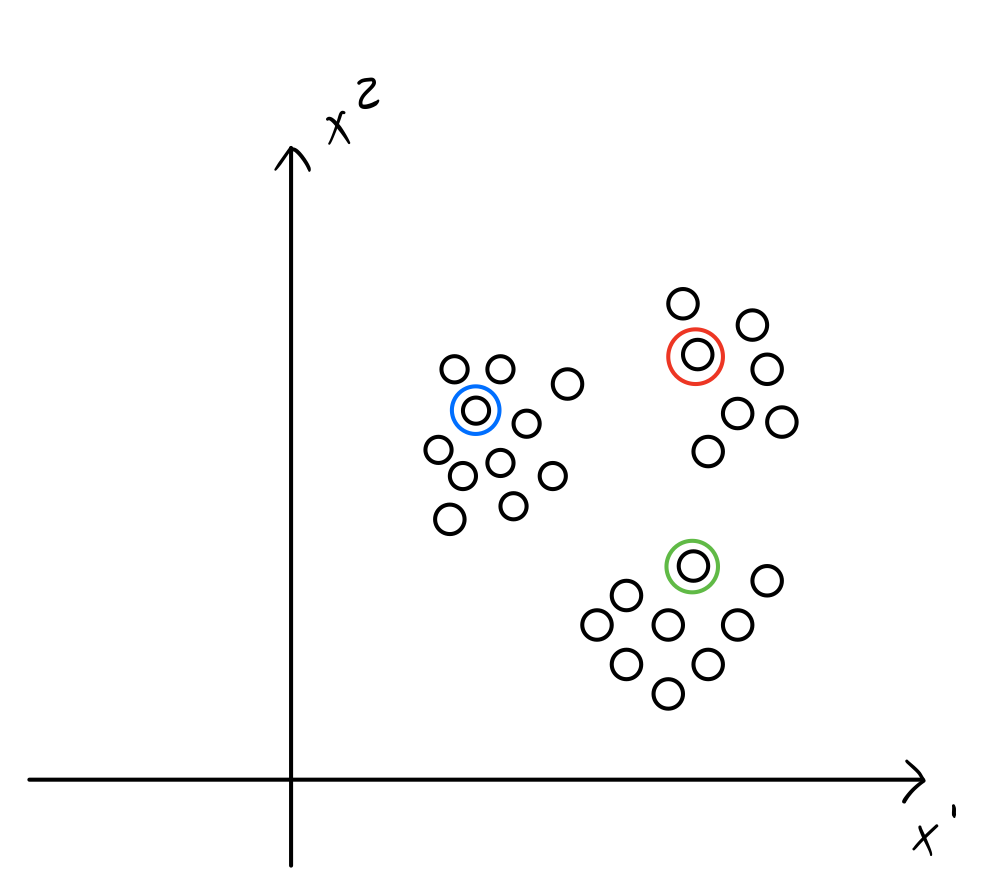
\includegraphics[scale=0.133]{./figs/KMeans_Fig2.png} &
	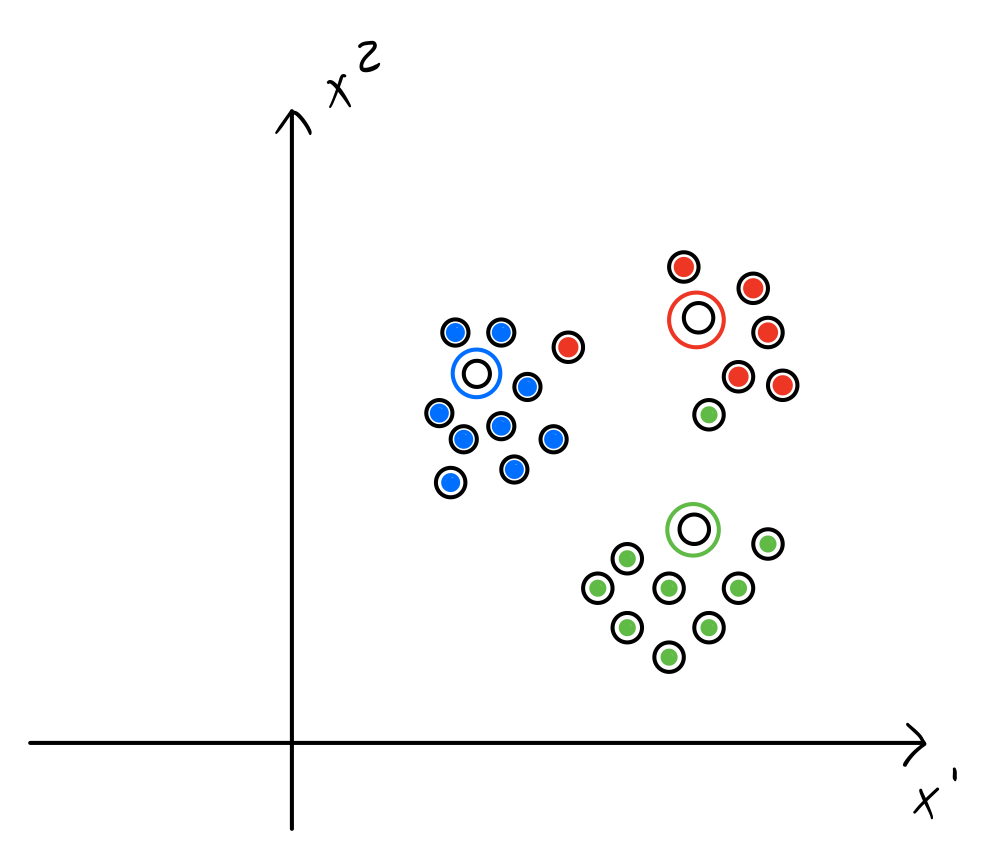
\includegraphics[scale=0.133]{./figs/KMeans_Fig3.png} &
	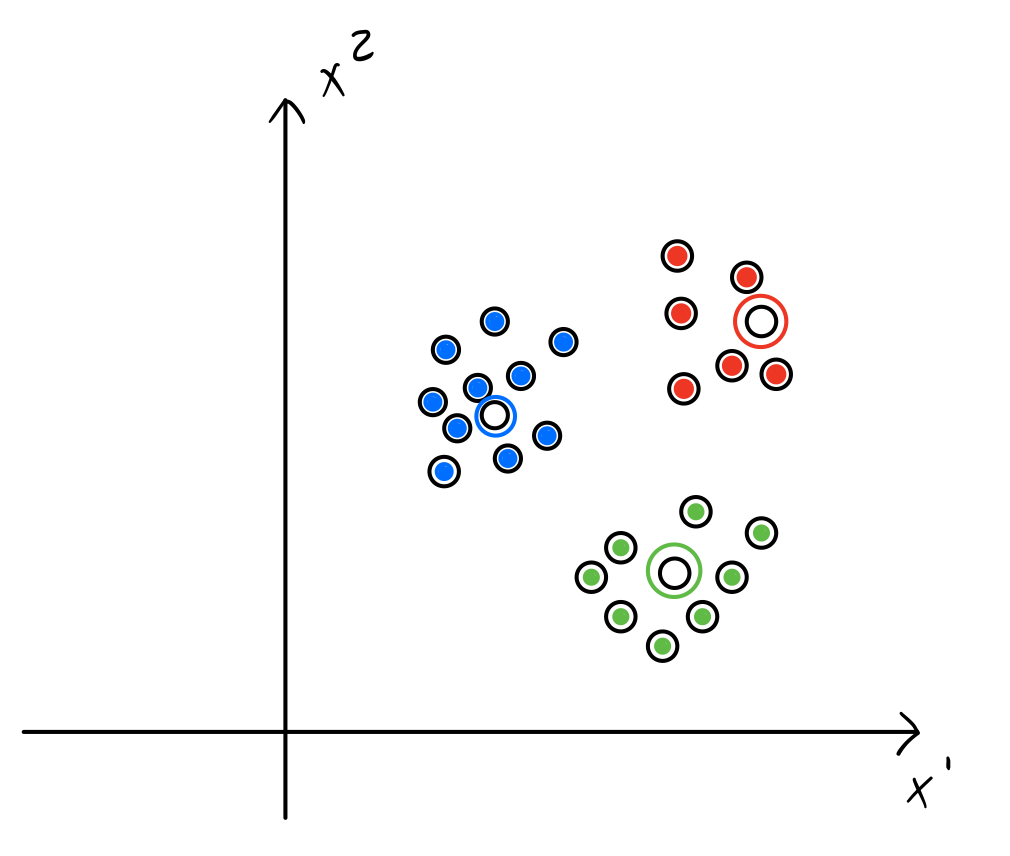
\includegraphics[scale=0.133]{./figs/KMeans_Fig4.png} \\
	Inicialização & Atribuição de centros & Configuração\\
	dos centros & mais próximos & final
\end{tabular}

}

\Sli{
\justifying Alguns pontos importantes:
\begin{itemize}
	\item Qual função de distância utilizar?
	\item Qual o valor de $k$?
	\item $k$-Médias assume assume que os agrupamentos são \textbf{circulamente simétricos} quando utilizamos a distância Euclidiana.
\end{itemize}
}

\end{document}